% Options for packages loaded elsewhere
\PassOptionsToPackage{unicode}{hyperref}
\PassOptionsToPackage{hyphens}{url}
%
\documentclass[
]{article}
\usepackage{lmodern}
\usepackage{amssymb,amsmath}
\usepackage{ifxetex,ifluatex}
\ifnum 0\ifxetex 1\fi\ifluatex 1\fi=0 % if pdftex
  \usepackage[T1]{fontenc}
  \usepackage[utf8]{inputenc}
  \usepackage{textcomp} % provide euro and other symbols
\else % if luatex or xetex
  \usepackage{unicode-math}
  \defaultfontfeatures{Scale=MatchLowercase}
  \defaultfontfeatures[\rmfamily]{Ligatures=TeX,Scale=1}
\fi
% Use upquote if available, for straight quotes in verbatim environments
\IfFileExists{upquote.sty}{\usepackage{upquote}}{}
\IfFileExists{microtype.sty}{% use microtype if available
  \usepackage[]{microtype}
  \UseMicrotypeSet[protrusion]{basicmath} % disable protrusion for tt fonts
}{}
\makeatletter
\@ifundefined{KOMAClassName}{% if non-KOMA class
  \IfFileExists{parskip.sty}{%
    \usepackage{parskip}
  }{% else
    \setlength{\parindent}{0pt}
    \setlength{\parskip}{6pt plus 2pt minus 1pt}}
}{% if KOMA class
  \KOMAoptions{parskip=half}}
\makeatother
\usepackage{xcolor}
\IfFileExists{xurl.sty}{\usepackage{xurl}}{} % add URL line breaks if available
\IfFileExists{bookmark.sty}{\usepackage{bookmark}}{\usepackage{hyperref}}
\hypersetup{
  pdftitle={STAT 428: Homework 5:   Chapter 7: Jackknife and Bootstrap},
  pdfauthor={Du, Yuting, yutingd3},
  hidelinks,
  pdfcreator={LaTeX via pandoc}}
\urlstyle{same} % disable monospaced font for URLs
\usepackage[margin=1in]{geometry}
\usepackage{color}
\usepackage{fancyvrb}
\newcommand{\VerbBar}{|}
\newcommand{\VERB}{\Verb[commandchars=\\\{\}]}
\DefineVerbatimEnvironment{Highlighting}{Verbatim}{commandchars=\\\{\}}
% Add ',fontsize=\small' for more characters per line
\usepackage{framed}
\definecolor{shadecolor}{RGB}{248,248,248}
\newenvironment{Shaded}{\begin{snugshade}}{\end{snugshade}}
\newcommand{\AlertTok}[1]{\textcolor[rgb]{0.94,0.16,0.16}{#1}}
\newcommand{\AnnotationTok}[1]{\textcolor[rgb]{0.56,0.35,0.01}{\textbf{\textit{#1}}}}
\newcommand{\AttributeTok}[1]{\textcolor[rgb]{0.77,0.63,0.00}{#1}}
\newcommand{\BaseNTok}[1]{\textcolor[rgb]{0.00,0.00,0.81}{#1}}
\newcommand{\BuiltInTok}[1]{#1}
\newcommand{\CharTok}[1]{\textcolor[rgb]{0.31,0.60,0.02}{#1}}
\newcommand{\CommentTok}[1]{\textcolor[rgb]{0.56,0.35,0.01}{\textit{#1}}}
\newcommand{\CommentVarTok}[1]{\textcolor[rgb]{0.56,0.35,0.01}{\textbf{\textit{#1}}}}
\newcommand{\ConstantTok}[1]{\textcolor[rgb]{0.00,0.00,0.00}{#1}}
\newcommand{\ControlFlowTok}[1]{\textcolor[rgb]{0.13,0.29,0.53}{\textbf{#1}}}
\newcommand{\DataTypeTok}[1]{\textcolor[rgb]{0.13,0.29,0.53}{#1}}
\newcommand{\DecValTok}[1]{\textcolor[rgb]{0.00,0.00,0.81}{#1}}
\newcommand{\DocumentationTok}[1]{\textcolor[rgb]{0.56,0.35,0.01}{\textbf{\textit{#1}}}}
\newcommand{\ErrorTok}[1]{\textcolor[rgb]{0.64,0.00,0.00}{\textbf{#1}}}
\newcommand{\ExtensionTok}[1]{#1}
\newcommand{\FloatTok}[1]{\textcolor[rgb]{0.00,0.00,0.81}{#1}}
\newcommand{\FunctionTok}[1]{\textcolor[rgb]{0.00,0.00,0.00}{#1}}
\newcommand{\ImportTok}[1]{#1}
\newcommand{\InformationTok}[1]{\textcolor[rgb]{0.56,0.35,0.01}{\textbf{\textit{#1}}}}
\newcommand{\KeywordTok}[1]{\textcolor[rgb]{0.13,0.29,0.53}{\textbf{#1}}}
\newcommand{\NormalTok}[1]{#1}
\newcommand{\OperatorTok}[1]{\textcolor[rgb]{0.81,0.36,0.00}{\textbf{#1}}}
\newcommand{\OtherTok}[1]{\textcolor[rgb]{0.56,0.35,0.01}{#1}}
\newcommand{\PreprocessorTok}[1]{\textcolor[rgb]{0.56,0.35,0.01}{\textit{#1}}}
\newcommand{\RegionMarkerTok}[1]{#1}
\newcommand{\SpecialCharTok}[1]{\textcolor[rgb]{0.00,0.00,0.00}{#1}}
\newcommand{\SpecialStringTok}[1]{\textcolor[rgb]{0.31,0.60,0.02}{#1}}
\newcommand{\StringTok}[1]{\textcolor[rgb]{0.31,0.60,0.02}{#1}}
\newcommand{\VariableTok}[1]{\textcolor[rgb]{0.00,0.00,0.00}{#1}}
\newcommand{\VerbatimStringTok}[1]{\textcolor[rgb]{0.31,0.60,0.02}{#1}}
\newcommand{\WarningTok}[1]{\textcolor[rgb]{0.56,0.35,0.01}{\textbf{\textit{#1}}}}
\usepackage{graphicx,grffile}
\makeatletter
\def\maxwidth{\ifdim\Gin@nat@width>\linewidth\linewidth\else\Gin@nat@width\fi}
\def\maxheight{\ifdim\Gin@nat@height>\textheight\textheight\else\Gin@nat@height\fi}
\makeatother
% Scale images if necessary, so that they will not overflow the page
% margins by default, and it is still possible to overwrite the defaults
% using explicit options in \includegraphics[width, height, ...]{}
\setkeys{Gin}{width=\maxwidth,height=\maxheight,keepaspectratio}
% Set default figure placement to htbp
\makeatletter
\def\fps@figure{htbp}
\makeatother
\setlength{\emergencystretch}{3em} % prevent overfull lines
\providecommand{\tightlist}{%
  \setlength{\itemsep}{0pt}\setlength{\parskip}{0pt}}
\setcounter{secnumdepth}{-\maxdimen} % remove section numbering
% https://github.com/rstudio/rmarkdown/issues/337
\let\rmarkdownfootnote\footnote%
\def\footnote{\protect\rmarkdownfootnote}

% https://github.com/rstudio/rmarkdown/pull/252
\usepackage{titling}
\setlength{\droptitle}{-2em}

\pretitle{\vspace{\droptitle}\centering\huge}
\posttitle{\par}

\preauthor{\centering\large\emph}
\postauthor{\par}

\predate{\centering\large\emph}
\postdate{\par}

\title{STAT 428: Homework 5: Chapter 7: Jackknife and Bootstrap}
\author{Du, Yuting, yutingd3}
\date{}

\begin{document}
\maketitle

{
\setcounter{tocdepth}{2}
\tableofcontents
}
\begin{center}\rule{0.5\linewidth}{\linethickness}\end{center}

Please refer to the {[}\textbf{detailed homework policy document}{]} on
Course Page for information about homework formatting, submission, and
grading.

\begin{center}\rule{0.5\linewidth}{\linethickness}\end{center}

\hypertarget{exercise-1}{%
\subsection{Exercise 1}\label{exercise-1}}

\textbf{Bootstrap (Normal).}

Perform the following tasks:

\begin{enumerate}
\def\labelenumi{\arabic{enumi}.}
\tightlist
\item
  Generate a sample of size 100 from \texttt{N(10,1)} distribution.
\end{enumerate}

\begin{Shaded}
\begin{Highlighting}[]
\NormalTok{n =}\StringTok{ }\DecValTok{100}
\NormalTok{x =}\StringTok{ }\KeywordTok{rnorm}\NormalTok{(n, }\DecValTok{10}\NormalTok{, }\DecValTok{1}\NormalTok{)}
\end{Highlighting}
\end{Shaded}

\begin{enumerate}
\def\labelenumi{\arabic{enumi}.}
\setcounter{enumi}{1}
\tightlist
\item
  Estimate the mean of observations in this sample.
\end{enumerate}

\begin{Shaded}
\begin{Highlighting}[]
\NormalTok{m =}\StringTok{ }\KeywordTok{mean}\NormalTok{(x)}
\end{Highlighting}
\end{Shaded}

\begin{enumerate}
\def\labelenumi{\arabic{enumi}.}
\setcounter{enumi}{2}
\tightlist
\item
  Use Bootstrap to estimate the standard error of this mean.
\end{enumerate}

\begin{Shaded}
\begin{Highlighting}[]
\NormalTok{B =}\StringTok{ }\DecValTok{10000}
\NormalTok{Tboot <-}\StringTok{ }\KeywordTok{numeric}\NormalTok{(B)}
\ControlFlowTok{for}\NormalTok{ (b }\ControlFlowTok{in} \DecValTok{1} \OperatorTok{:}\StringTok{ }\NormalTok{B) \{}
\NormalTok{  xb <-}\StringTok{ }\KeywordTok{sample}\NormalTok{(x, n, }\DataTypeTok{replace=}\OtherTok{TRUE}\NormalTok{)}
\NormalTok{  Tboot[b] <-}\StringTok{ }\KeywordTok{mean}\NormalTok{(xb)}
\NormalTok{\}}
\NormalTok{(se <-}\StringTok{ }\KeywordTok{sd}\NormalTok{(Tboot))}
\end{Highlighting}
\end{Shaded}

\begin{verbatim}
## [1] 0.1089
\end{verbatim}

\begin{enumerate}
\def\labelenumi{\arabic{enumi}.}
\setcounter{enumi}{3}
\tightlist
\item
  What should be (theoretically) and is (practically according to your
  experiment) the relation between this Bootstrap estimate and the
  actual standard deviation of the distribution you sampled from?
\end{enumerate}

\begin{Shaded}
\begin{Highlighting}[]
\NormalTok{norm_sd <-}\StringTok{ }\DecValTok{1} \OperatorTok{/}\StringTok{ }\DecValTok{5}
\NormalTok{(se_theory <-}\StringTok{ }\NormalTok{norm_sd }\OperatorTok{/}\StringTok{ }\KeywordTok{sqrt}\NormalTok{(n))}
\end{Highlighting}
\end{Shaded}

\begin{verbatim}
## [1] 0.02
\end{verbatim}

\begin{enumerate}
\def\labelenumi{\arabic{enumi}.}
\setcounter{enumi}{4}
\tightlist
\item
  Calculate a 95\% confidence interval for the estimate of mean (based
  on bootstrap).
\end{enumerate}

\begin{Shaded}
\begin{Highlighting}[]
\NormalTok{zval <-}\StringTok{ }\KeywordTok{qnorm}\NormalTok{(.}\DecValTok{975}\NormalTok{)}
\NormalTok{(lower <-}\StringTok{ }\NormalTok{m }\OperatorTok{-}\StringTok{ }\NormalTok{zval }\OperatorTok{*}\StringTok{ }\NormalTok{se)}
\end{Highlighting}
\end{Shaded}

\begin{verbatim}
## [1] 9.805
\end{verbatim}

\begin{Shaded}
\begin{Highlighting}[]
\NormalTok{(upper <-}\StringTok{ }\NormalTok{m }\OperatorTok{+}\StringTok{ }\NormalTok{zval }\OperatorTok{*}\StringTok{ }\NormalTok{se)}
\end{Highlighting}
\end{Shaded}

\begin{verbatim}
## [1] 10.23
\end{verbatim}

\hypertarget{exercise-2}{%
\subsection{Exercise 2}\label{exercise-2}}

\textbf{Jackknife (Normal).}

Consider the same sample that you generated in Exercise 1.1 and the same
estimator you used in Exercise 1.2. Find the jackknife estimate of the
bias of this estimator. (You may choose to guess the answer instead of
performing the jackknife procedure, in that case EXPLAIN clearly why
your guess makes sense.)

\begin{verbatim}
## [1] -0.0002328  0.0217774
\end{verbatim}

The bias is about -0.0002536.

\hypertarget{exercise-3}{%
\subsection{Exercise 3}\label{exercise-3}}

\textbf{Bootstrap and Jackknife Error Comparison} Consider the following
(simulated) months until various batteries of the same type burn out:

\begin{Shaded}
\begin{Highlighting}[]
\NormalTok{Ex3 <-}\StringTok{ }\KeywordTok{c}\NormalTok{(}\FloatTok{2.228}\NormalTok{, }\FloatTok{2.051}\NormalTok{, }\FloatTok{1.683}\NormalTok{, }\FloatTok{3.285}\NormalTok{, }\FloatTok{1.219}\NormalTok{, }\FloatTok{2.879}\NormalTok{, }\FloatTok{2.976}\NormalTok{, }\FloatTok{2.112}\NormalTok{, }\FloatTok{2.357}\NormalTok{, }\FloatTok{2.425}\NormalTok{, }\FloatTok{1.255}\NormalTok{, }\FloatTok{2.562}\NormalTok{, }\FloatTok{0.829}\NormalTok{, }\FloatTok{2.581}\NormalTok{, }\FloatTok{2.340}\NormalTok{, }\FloatTok{3.043}\NormalTok{, }\FloatTok{0.684}\NormalTok{, }\FloatTok{1.810}\NormalTok{, }\FloatTok{2.529}\NormalTok{, }\FloatTok{0.700}\NormalTok{)}
\end{Highlighting}
\end{Shaded}

\begin{enumerate}
\def\labelenumi{\arabic{enumi}.}
\tightlist
\item
  We want to estimate the probability that these batteries burn out in
  less than 2 months, so \(\theta=P(X<2)\). Calculate \(\hat{\theta}\).
\end{enumerate}

\begin{Shaded}
\begin{Highlighting}[]
\NormalTok{count =}\StringTok{ }\DecValTok{0}
\ControlFlowTok{for}\NormalTok{(val }\ControlFlowTok{in}\NormalTok{ Ex3)\{}
  \ControlFlowTok{if}\NormalTok{(val }\OperatorTok{<}\StringTok{ }\DecValTok{2}\NormalTok{) count =}\StringTok{ }\NormalTok{count }\OperatorTok{+}\StringTok{ }\DecValTok{1}
\NormalTok{\}}

\NormalTok{theta.hat =}\StringTok{ }\NormalTok{count }\OperatorTok{/}\StringTok{ }\KeywordTok{length}\NormalTok{(Ex3)}
\NormalTok{theta.hat}
\end{Highlighting}
\end{Shaded}

\begin{verbatim}
## [1] 0.35
\end{verbatim}

\begin{enumerate}
\def\labelenumi{\arabic{enumi}.}
\setcounter{enumi}{1}
\tightlist
\item
  What is the standard error and bias of your estimator? Estimate the
  standard error and bias using bootstrapping.
\end{enumerate}

\begin{Shaded}
\begin{Highlighting}[]
\KeywordTok{library}\NormalTok{(SimDesign)}
\NormalTok{B =}\StringTok{ }\DecValTok{10000}
\NormalTok{Tboot <-}\StringTok{ }\KeywordTok{numeric}\NormalTok{(B)}
\ControlFlowTok{for}\NormalTok{ (b }\ControlFlowTok{in} \DecValTok{1} \OperatorTok{:}\StringTok{ }\NormalTok{B) \{}
\NormalTok{  xb <-}\StringTok{ }\KeywordTok{sample}\NormalTok{(Ex3, }\KeywordTok{length}\NormalTok{(Ex3), }\DataTypeTok{replace=}\OtherTok{TRUE}\NormalTok{)}
  
\NormalTok{  count =}\StringTok{ }\DecValTok{0}
  \ControlFlowTok{for}\NormalTok{(val }\ControlFlowTok{in}\NormalTok{ xb)\{}
    \ControlFlowTok{if}\NormalTok{(val }\OperatorTok{<}\StringTok{ }\DecValTok{2}\NormalTok{) count =}\StringTok{ }\NormalTok{count }\OperatorTok{+}\StringTok{ }\DecValTok{1}
\NormalTok{  \}}
  
\NormalTok{  Tboot[b] <-}\StringTok{ }\NormalTok{count }\OperatorTok{/}\StringTok{ }\KeywordTok{length}\NormalTok{(Ex3)}
\NormalTok{\}}
\NormalTok{(se <-}\StringTok{ }\KeywordTok{sd}\NormalTok{(Tboot))}
\end{Highlighting}
\end{Shaded}

\begin{verbatim}
## [1] 0.1063
\end{verbatim}

\begin{Shaded}
\begin{Highlighting}[]
\NormalTok{(bs <-}\StringTok{ }\KeywordTok{bias}\NormalTok{(Tboot))}
\end{Highlighting}
\end{Shaded}

\begin{verbatim}
## [1] 0.3517
\end{verbatim}

\begin{enumerate}
\def\labelenumi{\arabic{enumi}.}
\setcounter{enumi}{2}
\tightlist
\item
  Calculate the standard error and bias using Jackknife.
\end{enumerate}

\begin{Shaded}
\begin{Highlighting}[]
\KeywordTok{library}\NormalTok{(SimDesign)}
\NormalTok{B =}\StringTok{ }\DecValTok{10000}
\NormalTok{x <-}\StringTok{ }\KeywordTok{numeric}\NormalTok{()}
\ControlFlowTok{for}\NormalTok{ (b }\ControlFlowTok{in} \DecValTok{1} \OperatorTok{:}\StringTok{ }\NormalTok{B) \{}
\NormalTok{  x[b] <-}\StringTok{ }\KeywordTok{sample}\NormalTok{(Ex3, }\KeywordTok{length}\NormalTok{(Ex3), }\DataTypeTok{replace=}\OtherTok{TRUE}\NormalTok{)}\CommentTok{#the data}
\NormalTok{\}}

\NormalTok{theta.hat =}\StringTok{ }\KeywordTok{mean}\NormalTok{(x}\OperatorTok{<}\DecValTok{2}\NormalTok{)}\CommentTok{#the estimate}
\NormalTok{theta.hat.jack =}\StringTok{ }\KeywordTok{numeric}\NormalTok{()}

\ControlFlowTok{for}\NormalTok{(i }\ControlFlowTok{in} \DecValTok{1}\OperatorTok{:}\StringTok{ }\NormalTok{B)\{}
\NormalTok{  xi =}\StringTok{ }\NormalTok{x[}\OperatorTok{-}\NormalTok{i]}
\NormalTok{  theta.hat.jack[i] =}\StringTok{ }\KeywordTok{mean}\NormalTok{(xi}\OperatorTok{<}\DecValTok{2}\NormalTok{)}
\NormalTok{\}}

\CommentTok{#Calculate standard error}
\NormalTok{sumsq=}\KeywordTok{sum}\NormalTok{((theta.hat.jack}\OperatorTok{-}\KeywordTok{mean}\NormalTok{(theta.hat.jack))}\OperatorTok{^}\DecValTok{2}\NormalTok{)}
\KeywordTok{sqrt}\NormalTok{((n}\DecValTok{-1}\NormalTok{)}\OperatorTok{/}\NormalTok{n)}\OperatorTok{*}\KeywordTok{sqrt}\NormalTok{(sumsq)}
\end{Highlighting}
\end{Shaded}

\begin{verbatim}
## [1] 0.004738
\end{verbatim}

\begin{Shaded}
\begin{Highlighting}[]
\CommentTok{#Calculate bias}
\NormalTok{(n}\DecValTok{-1}\NormalTok{)}\OperatorTok{*}\NormalTok{(}\KeywordTok{mean}\NormalTok{(theta.hat.jack)}\OperatorTok{-}\NormalTok{theta.hat)}
\end{Highlighting}
\end{Shaded}

\begin{verbatim}
## [1] 0
\end{verbatim}

\begin{enumerate}
\def\labelenumi{\arabic{enumi}.}
\setcounter{enumi}{3}
\tightlist
\item
  What if you wanted to calculate the median time to burn out instead?
  Estimate the median, the standard error of the median estimator, and
  the bias of the median estimator using a resampling method.
\end{enumerate}

\begin{Shaded}
\begin{Highlighting}[]
\KeywordTok{library}\NormalTok{(SimDesign)}
\NormalTok{B =}\StringTok{ }\DecValTok{10000}
\NormalTok{Tboot <-}\StringTok{ }\KeywordTok{numeric}\NormalTok{()}
\ControlFlowTok{for}\NormalTok{ (b }\ControlFlowTok{in} \DecValTok{1} \OperatorTok{:}\StringTok{ }\NormalTok{B) \{}
\NormalTok{  xb <-}\StringTok{ }\KeywordTok{sample}\NormalTok{(Ex3, }\KeywordTok{length}\NormalTok{(Ex3), }\DataTypeTok{replace=}\OtherTok{TRUE}\NormalTok{)}
\NormalTok{  Tboot[b] <-}\StringTok{ }\KeywordTok{median}\NormalTok{(xb)}
\NormalTok{\}}
\NormalTok{(se <-}\StringTok{ }\KeywordTok{sd}\NormalTok{(Tboot))}
\end{Highlighting}
\end{Shaded}

\begin{verbatim}
## [1] 0.2031
\end{verbatim}

\begin{Shaded}
\begin{Highlighting}[]
\NormalTok{(bs <-}\StringTok{ }\KeywordTok{bias}\NormalTok{(Tboot))}
\end{Highlighting}
\end{Shaded}

\begin{verbatim}
## [1] 2.239
\end{verbatim}

\hypertarget{exercise-4}{%
\subsection{Exercise 4}\label{exercise-4}}

Consider the data stored in \texttt{cw} on the weight of 30 chicks after
eating two different diets for ten days. Chicks 1-20 had diet 1, and
chicks 21-30 had diet 2.

\begin{Shaded}
\begin{Highlighting}[]
\NormalTok{cw<-ChickWeight[ChickWeight}\OperatorTok{$}\NormalTok{Time}\OperatorTok{==}\DecValTok{10}\OperatorTok{&}\NormalTok{ChickWeight}\OperatorTok{$}\NormalTok{Diet }\OperatorTok\StringTok{ }\KeywordTok{c}\NormalTok{(}\StringTok{"1"}\NormalTok{,}\StringTok{"2"}\NormalTok{),]}
\NormalTok{cw<-}\KeywordTok{droplevels}\NormalTok{(cw)}
\end{Highlighting}
\end{Shaded}

Using a permutation test, determine whether the mean weights of the
chicks on the two diets are different. Clearly show your steps, with at
least comments to explain what you are doing (you should be doing this
anyway, but just a reminder). What do you conclude?

\begin{Shaded}
\begin{Highlighting}[]
\NormalTok{x =}\StringTok{ }\NormalTok{cw[}\StringTok{"weight"}\NormalTok{][cw[}\StringTok{"Diet"}\NormalTok{] }\OperatorTok{==}\StringTok{ }\DecValTok{1}\NormalTok{]}
\NormalTok{y =}\StringTok{ }\NormalTok{cw[}\StringTok{"weight"}\NormalTok{][cw[}\StringTok{"Diet"}\NormalTok{] }\OperatorTok{==}\StringTok{ }\DecValTok{2}\NormalTok{]}

\CommentTok{# First we find the p-value for the two-sample t statistic by referring to thet-distribution with n+m-2 df}
\KeywordTok{t.test}\NormalTok{(x,y,}\DataTypeTok{var.equal=}\OtherTok{TRUE}\NormalTok{)}
\end{Highlighting}
\end{Shaded}

\begin{verbatim}
## 
##  Two Sample t-test
## 
## data:  x and y
## t = -1.7, df = 27, p-value = 0.1
## alternative hypothesis: true difference in means is not equal to 0
## 95 percent confidence interval:
##  -33.998   3.103
## sample estimates:
## mean of x mean of y 
##     93.05    108.50
\end{verbatim}

\begin{Shaded}
\begin{Highlighting}[]
\CommentTok{# Now we’ll let θˆ = |t| to test null hypothesis}
\CommentTok{# of equal mean against a two sided alternative,}
\CommentTok{# and use the randomization distribution for the}
\CommentTok{# p-value}
\NormalTok{x =}\StringTok{ }\KeywordTok{c}\NormalTok{(cw[}\StringTok{"weight"}\NormalTok{][cw[}\StringTok{"Diet"}\NormalTok{] }\OperatorTok{==}\StringTok{ }\DecValTok{1}\NormalTok{])}
\NormalTok{y =}\StringTok{ }\KeywordTok{c}\NormalTok{(cw[}\StringTok{"weight"}\NormalTok{][cw[}\StringTok{"Diet"}\NormalTok{] }\OperatorTok{==}\StringTok{ }\DecValTok{2}\NormalTok{])}

\NormalTok{B =}\StringTok{ }\DecValTok{1000} \CommentTok{#The number of bootstrap samples to take}
\NormalTok{z =}\StringTok{ }\KeywordTok{c}\NormalTok{(x,y)}
\NormalTok{nu =}\StringTok{ }\DecValTok{1}\OperatorTok{:}\KeywordTok{length}\NormalTok{(z)}
\NormalTok{reps=}\KeywordTok{numeric}\NormalTok{(B)}
\NormalTok{t0=}\KeywordTok{t.test}\NormalTok{(x,y,}\DataTypeTok{var.equal=}\OtherTok{FALSE}\NormalTok{)}\OperatorTok{$}\NormalTok{statistic}
\ControlFlowTok{for}\NormalTok{(i }\ControlFlowTok{in} \DecValTok{1}\OperatorTok{:}\NormalTok{B)\{}
\NormalTok{  perm=}\KeywordTok{sample}\NormalTok{(nu,}\DataTypeTok{size=}\KeywordTok{length}\NormalTok{(x),}\DataTypeTok{replace=}\OtherTok{FALSE}\NormalTok{)}
\NormalTok{  x1=z[perm]}
\NormalTok{  y1=z[}\OperatorTok{-}\NormalTok{perm]}
\NormalTok{  reps[i]=}\KeywordTok{abs}\NormalTok{(}\KeywordTok{t.test}\NormalTok{(x1,y1,}\DataTypeTok{var.equal=}\OtherTok{FALSE}\NormalTok{)}\OperatorTok{$}\NormalTok{statistic)}
\NormalTok{\}}
\KeywordTok{mean}\NormalTok{(}\KeywordTok{c}\NormalTok{(t0,reps)}\OperatorTok{>=}\NormalTok{t0)}
\end{Highlighting}
\end{Shaded}

\begin{verbatim}
## [1] 1
\end{verbatim}

So, the two means are quite similar.

\hypertarget{exercise-5}{%
\subsection{Exercise 5}\label{exercise-5}}

Do exercise 7.3 from the book.

7.3 Obtain a bootstrap t confidence interval estimate for the
correlation statistic in Example 7.2 (law data in bootstrap).

\begin{Shaded}
\begin{Highlighting}[]
\KeywordTok{library}\NormalTok{(}\StringTok{"bootstrap"}\NormalTok{)}
\NormalTok{B =}\StringTok{ }\DecValTok{200}
\NormalTok{n =}\StringTok{ }\KeywordTok{nrow}\NormalTok{(law)}

\NormalTok{theta.hat =}\StringTok{ }\KeywordTok{cor}\NormalTok{(law}\OperatorTok{$}\NormalTok{LSAT, law}\OperatorTok{$}\NormalTok{GPA)}
\NormalTok{theta.hats.b =}\StringTok{ }\KeywordTok{numeric}\NormalTok{(B)}

\NormalTok{ts =}\StringTok{ }\KeywordTok{numeric}\NormalTok{(B)}

\ControlFlowTok{for}\NormalTok{ (b }\ControlFlowTok{in} \DecValTok{1}\OperatorTok{:}\NormalTok{B) \{}
\NormalTok{  i =}\StringTok{ }\KeywordTok{sample}\NormalTok{(}\DataTypeTok{x =} \DecValTok{1}\OperatorTok{:}\NormalTok{n, }\DataTypeTok{size =}\NormalTok{ n, }\DataTypeTok{replace =} \OtherTok{TRUE}\NormalTok{)}
\NormalTok{  law.b =}\StringTok{ }\NormalTok{law[i,]}
\NormalTok{  theta.hats.b[b] =}\StringTok{ }\KeywordTok{cor}\NormalTok{(law.b}\OperatorTok{$}\NormalTok{LSAT, law.b}\OperatorTok{$}\NormalTok{GPA)}
\NormalTok{  sd.theta.hats.b =}\StringTok{ }\KeywordTok{numeric}\NormalTok{(B)}
  
  \ControlFlowTok{for}\NormalTok{(b2 }\ControlFlowTok{in} \DecValTok{1}\OperatorTok{:}\NormalTok{B) \{}
\NormalTok{    i2 =}\StringTok{ }\KeywordTok{sample}\NormalTok{(}\DataTypeTok{x =} \DecValTok{1}\OperatorTok{:}\NormalTok{n, }\DataTypeTok{size =}\NormalTok{ n, }\DataTypeTok{replace =} \OtherTok{TRUE}\NormalTok{)}
\NormalTok{    law.b2 =}\StringTok{ }\NormalTok{law.b[i2,]}
\NormalTok{    sd.theta.hats.b[b2] =}\StringTok{ }\KeywordTok{cor}\NormalTok{(law.b2}\OperatorTok{$}\NormalTok{LSAT, law.b2}\OperatorTok{$}\NormalTok{GPA)}
\NormalTok{  \}}
  
\NormalTok{  se.b =}\StringTok{ }\KeywordTok{sd}\NormalTok{(sd.theta.hats.b)}
  
\NormalTok{  ts[b] =}\StringTok{ }\NormalTok{(theta.hats.b[b] }\OperatorTok{-}\StringTok{ }\NormalTok{theta.hat) }\OperatorTok{/}\StringTok{ }\NormalTok{se.b}
\NormalTok{\}}

\NormalTok{alpha =}\StringTok{ }\FloatTok{0.05}
\NormalTok{ts.ordered =}\StringTok{ }\KeywordTok{sort}\NormalTok{(ts)}

\NormalTok{qs =}\StringTok{ }\KeywordTok{quantile}\NormalTok{(ts.ordered, }\DataTypeTok{probs =} \KeywordTok{c}\NormalTok{(alpha}\OperatorTok{/}\DecValTok{2}\NormalTok{, }\DecValTok{1}\OperatorTok{-}\NormalTok{alpha}\OperatorTok{/}\DecValTok{2}\NormalTok{))}

\NormalTok{se.hat =}\StringTok{ }\KeywordTok{sd}\NormalTok{(theta.hats.b)}

\NormalTok{(}\DataTypeTok{CI =} \KeywordTok{c}\NormalTok{(theta.hat }\OperatorTok{-}\StringTok{ }\NormalTok{qs[}\DecValTok{2}\NormalTok{]}\OperatorTok{*}\NormalTok{se.hat, theta.hat }\OperatorTok{-}\StringTok{ }\NormalTok{qs[}\DecValTok{1}\NormalTok{]}\OperatorTok{*}\NormalTok{se.hat))}
\end{Highlighting}
\end{Shaded}

\begin{verbatim}
##   97.5%    2.5% 
## -0.2897  0.9694
\end{verbatim}

\begin{Shaded}
\begin{Highlighting}[]
\KeywordTok{hist}\NormalTok{(ts, }\DataTypeTok{breaks =} \DecValTok{100}\NormalTok{, }\DataTypeTok{xlim =} \KeywordTok{c}\NormalTok{(}\OperatorTok{-}\DecValTok{5}\NormalTok{, }\DecValTok{10}\NormalTok{))}
\end{Highlighting}
\end{Shaded}

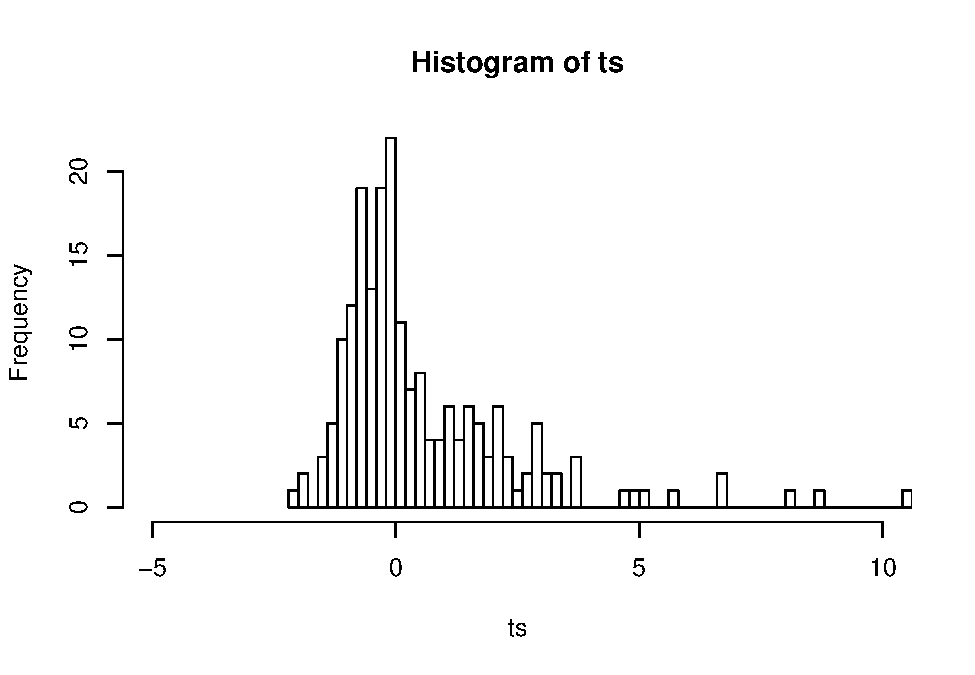
\includegraphics{428HW5-yutingd3_files/figure-latex/unnamed-chunk-15-1.pdf}

\hypertarget{exercise-6}{%
\subsection{Exercise 6}\label{exercise-6}}

Do exercise 7.10 from the book.

7.10 In Example 7.18, leave-one-out (n-fold) cross validation was used
to select the best fitting model. Repeat the analysis replacing the
Log-Log model with a cubic polynomial model. Which of the four models is
selected by the cross validation procedure? Which model is selected
according to maximus adjusted \(R^2\)?

\begin{Shaded}
\begin{Highlighting}[]
\KeywordTok{library}\NormalTok{(DAAG); }\KeywordTok{attach}\NormalTok{(ironslag)}

\NormalTok{n <-}\StringTok{ }\KeywordTok{length}\NormalTok{(magnetic) }\CommentTok{#in DAAG ironslag}
\NormalTok{e1 <-}\StringTok{ }\NormalTok{e2 <-}\StringTok{ }\NormalTok{e3 <-}\StringTok{ }\NormalTok{e4 <-}\StringTok{ }\KeywordTok{numeric}\NormalTok{(n)}
\CommentTok{# for n-fold cross validation}
\CommentTok{# fit models on leave-one-out samples}
\ControlFlowTok{for}\NormalTok{ (k }\ControlFlowTok{in} \DecValTok{1}\OperatorTok{:}\NormalTok{n) \{}
\NormalTok{y <-}\StringTok{ }\NormalTok{magnetic[}\OperatorTok{-}\NormalTok{k]}
\NormalTok{x <-}\StringTok{ }\NormalTok{chemical[}\OperatorTok{-}\NormalTok{k]}
\NormalTok{J1 <-}\StringTok{ }\KeywordTok{lm}\NormalTok{(y }\OperatorTok{~}\StringTok{ }\NormalTok{x)}
\NormalTok{yhat1 <-}\StringTok{ }\NormalTok{J1}\OperatorTok{$}\NormalTok{coef[}\DecValTok{1}\NormalTok{] }\OperatorTok{+}\StringTok{ }\NormalTok{J1}\OperatorTok{$}\NormalTok{coef[}\DecValTok{2}\NormalTok{] }\OperatorTok{*}\StringTok{ }\NormalTok{chemical[k]}
\NormalTok{e1[k] <-}\StringTok{ }\NormalTok{magnetic[k] }\OperatorTok{-}\StringTok{ }\NormalTok{yhat1}

\NormalTok{J2 <-}\StringTok{ }\KeywordTok{lm}\NormalTok{(y }\OperatorTok{~}\StringTok{ }\NormalTok{x }\OperatorTok{+}\StringTok{ }\KeywordTok{I}\NormalTok{(x}\OperatorTok{^}\DecValTok{2}\NormalTok{) }\OperatorTok{+}\StringTok{ }\KeywordTok{I}\NormalTok{(x}\OperatorTok{^}\DecValTok{3}\NormalTok{))}
\NormalTok{yhat2 <-}\StringTok{ }\NormalTok{J2}\OperatorTok{$}\NormalTok{coef[}\DecValTok{1}\NormalTok{] }\OperatorTok{+}\StringTok{ }\NormalTok{J2}\OperatorTok{$}\NormalTok{coef[}\DecValTok{2}\NormalTok{] }\OperatorTok{*}\StringTok{ }\NormalTok{chemical[k] }\OperatorTok{+}
\NormalTok{J2}\OperatorTok{$}\NormalTok{coef[}\DecValTok{3}\NormalTok{] }\OperatorTok{*}\StringTok{ }\NormalTok{chemical[k]}\OperatorTok{^}\DecValTok{2} \OperatorTok{+}\StringTok{ }\NormalTok{J2}\OperatorTok{$}\NormalTok{coef[}\DecValTok{4}\NormalTok{] }\OperatorTok{*}\StringTok{ }\NormalTok{chemical[k]}\OperatorTok{^}\DecValTok{3}
\NormalTok{e2[k] <-}\StringTok{ }\NormalTok{magnetic[k] }\OperatorTok{-}\StringTok{ }\NormalTok{yhat2}

\NormalTok{J3 <-}\StringTok{ }\KeywordTok{lm}\NormalTok{(}\KeywordTok{log}\NormalTok{(y) }\OperatorTok{~}\StringTok{ }\NormalTok{x)}
\NormalTok{logyhat3 <-}\StringTok{ }\NormalTok{J3}\OperatorTok{$}\NormalTok{coef[}\DecValTok{1}\NormalTok{] }\OperatorTok{+}\StringTok{ }\NormalTok{J3}\OperatorTok{$}\NormalTok{coef[}\DecValTok{2}\NormalTok{] }\OperatorTok{*}\StringTok{ }\NormalTok{chemical[k]}
\NormalTok{yhat3 <-}\StringTok{ }\KeywordTok{exp}\NormalTok{(logyhat3)}
\NormalTok{e3[k] <-}\StringTok{ }\NormalTok{magnetic[k] }\OperatorTok{-}\StringTok{ }\NormalTok{yhat3}

\NormalTok{J4 <-}\StringTok{ }\KeywordTok{lm}\NormalTok{(}\KeywordTok{log}\NormalTok{(y) }\OperatorTok{~}\StringTok{ }\KeywordTok{log}\NormalTok{(x))}
\NormalTok{logyhat4 <-}\StringTok{ }\NormalTok{J4}\OperatorTok{$}\NormalTok{coef[}\DecValTok{1}\NormalTok{] }\OperatorTok{+}\StringTok{ }\NormalTok{J4}\OperatorTok{$}\NormalTok{coef[}\DecValTok{2}\NormalTok{] }\OperatorTok{*}\StringTok{ }\KeywordTok{log}\NormalTok{(chemical[k])}
\NormalTok{yhat4 <-}\StringTok{ }\KeywordTok{exp}\NormalTok{(logyhat4)}
\NormalTok{e4[k] <-}\StringTok{ }\NormalTok{magnetic[k] }\OperatorTok{-}\StringTok{ }\NormalTok{yhat4}
\NormalTok{\}}

\KeywordTok{c}\NormalTok{(}\KeywordTok{mean}\NormalTok{(e1}\OperatorTok{^}\DecValTok{2}\NormalTok{), }\KeywordTok{mean}\NormalTok{(e2}\OperatorTok{^}\DecValTok{2}\NormalTok{), }\KeywordTok{mean}\NormalTok{(e3}\OperatorTok{^}\DecValTok{2}\NormalTok{), }\KeywordTok{mean}\NormalTok{(e4}\OperatorTok{^}\DecValTok{2}\NormalTok{))}
\end{Highlighting}
\end{Shaded}

\begin{verbatim}
## [1] 19.56 18.18 18.44 20.45
\end{verbatim}

According to the estimates for prediction error,the cubic model is best
fit for data. Then it's the exponential model, then the linear model.
The Log-log model is the worst.

\hypertarget{exercise-7}{%
\subsection{Exercise 7}\label{exercise-7}}

Do exercise 7.11 from the book.

7.11 In Example 7.18, leave-one-out (n-fold) cross validation was used
to select the best fitting model. Use leave-two-out cross validation to
compare the models.

\begin{Shaded}
\begin{Highlighting}[]
\KeywordTok{library}\NormalTok{(DAAG); }
\KeywordTok{attach}\NormalTok{(ironslag)}
\NormalTok{n <-}\StringTok{ }\KeywordTok{length}\NormalTok{(magnetic) }\CommentTok{#in DAAG ironslag}
\NormalTok{e1 <-}\StringTok{ }\NormalTok{e2 <-}\StringTok{ }\NormalTok{e3 <-}\StringTok{ }\NormalTok{e4 <-}\StringTok{ }\KeywordTok{numeric}\NormalTok{(n}\OperatorTok{*}\NormalTok{(n}\DecValTok{-1}\NormalTok{)) }\CommentTok{# 'leave two out' has n(n-1) combinations}

\ControlFlowTok{for}\NormalTok{ (i }\ControlFlowTok{in} \DecValTok{1}\OperatorTok{:}\NormalTok{n)\{}
  \ControlFlowTok{for}\NormalTok{ (j }\ControlFlowTok{in}\NormalTok{ i}\OperatorTok{:}\NormalTok{n)\{}
    \ControlFlowTok{if}\NormalTok{ (i }\OperatorTok{!=}\StringTok{ }\NormalTok{j)\{}
\NormalTok{      y=magnetic[}\KeywordTok{c}\NormalTok{(}\OperatorTok{-}\NormalTok{i,}\OperatorTok{-}\NormalTok{j)]}
\NormalTok{      x=chemical[}\KeywordTok{c}\NormalTok{(}\OperatorTok{-}\NormalTok{i,}\OperatorTok{-}\NormalTok{j)]}
      
\NormalTok{      J1 <-}\StringTok{ }\KeywordTok{lm}\NormalTok{(y }\OperatorTok{~}\StringTok{ }\NormalTok{x)}
\NormalTok{      yhat11 <-}\StringTok{ }\NormalTok{J1}\OperatorTok{$}\NormalTok{coef[}\DecValTok{1}\NormalTok{] }\OperatorTok{+}\StringTok{ }\NormalTok{J1}\OperatorTok{$}\NormalTok{coef[}\DecValTok{2}\NormalTok{] }\OperatorTok{*}\StringTok{ }\NormalTok{chemical[i]}
\NormalTok{      yhat12 <-}\StringTok{ }\NormalTok{J1}\OperatorTok{$}\NormalTok{coef[}\DecValTok{1}\NormalTok{] }\OperatorTok{+}\StringTok{ }\NormalTok{J1}\OperatorTok{$}\NormalTok{coef[}\DecValTok{2}\NormalTok{] }\OperatorTok{*}\StringTok{ }\NormalTok{chemical[j]}
\NormalTok{      e1[(i}\DecValTok{-1}\NormalTok{)}\OperatorTok{*}\NormalTok{n}\OperatorTok{+}\NormalTok{j] <-}\StringTok{ }\KeywordTok{sqrt}\NormalTok{((magnetic[i] }\OperatorTok{-}\StringTok{ }\NormalTok{yhat11)}\OperatorTok{^}\DecValTok{2}\OperatorTok{+}\NormalTok{(magnetic[j] }\OperatorTok{-}\StringTok{ }\NormalTok{yhat12)}\OperatorTok{^}\DecValTok{2}\NormalTok{)}
      
\NormalTok{      J2 <-}\StringTok{ }\KeywordTok{lm}\NormalTok{(y }\OperatorTok{~}\StringTok{ }\NormalTok{x }\OperatorTok{+}\StringTok{ }\KeywordTok{I}\NormalTok{(x}\OperatorTok{^}\DecValTok{2}\NormalTok{))}
\NormalTok{      yhat21 <-}\StringTok{ }\NormalTok{J2}\OperatorTok{$}\NormalTok{coef[}\DecValTok{1}\NormalTok{] }\OperatorTok{+}\StringTok{ }\NormalTok{J2}\OperatorTok{$}\NormalTok{coef[}\DecValTok{2}\NormalTok{] }\OperatorTok{*}\StringTok{ }\NormalTok{chemical[i] }\OperatorTok{+}
\StringTok{      }\NormalTok{J2}\OperatorTok{$}\NormalTok{coef[}\DecValTok{3}\NormalTok{] }\OperatorTok{*}\StringTok{ }\NormalTok{chemical[i]}\OperatorTok{^}\DecValTok{2}
\NormalTok{      yhat22 <-}\StringTok{ }\NormalTok{J2}\OperatorTok{$}\NormalTok{coef[}\DecValTok{1}\NormalTok{] }\OperatorTok{+}\StringTok{ }\NormalTok{J2}\OperatorTok{$}\NormalTok{coef[}\DecValTok{2}\NormalTok{] }\OperatorTok{*}\StringTok{ }\NormalTok{chemical[j] }\OperatorTok{+}
\StringTok{      }\NormalTok{J2}\OperatorTok{$}\NormalTok{coef[}\DecValTok{3}\NormalTok{] }\OperatorTok{*}\StringTok{ }\NormalTok{chemical[j]}\OperatorTok{^}\DecValTok{2}
\NormalTok{      e2[(i}\DecValTok{-1}\NormalTok{)}\OperatorTok{*}\NormalTok{n}\OperatorTok{+}\NormalTok{j] <-}\StringTok{ }\KeywordTok{sqrt}\NormalTok{((magnetic[i] }\OperatorTok{-}\StringTok{ }\NormalTok{yhat21)}\OperatorTok{^}\DecValTok{2}\OperatorTok{+}\NormalTok{(magnetic[j] }\OperatorTok{-}\StringTok{ }\NormalTok{yhat22)}\OperatorTok{^}\DecValTok{2}\NormalTok{)}
      
\NormalTok{      J3 <-}\StringTok{ }\KeywordTok{lm}\NormalTok{(}\KeywordTok{log}\NormalTok{(y) }\OperatorTok{~}\StringTok{ }\NormalTok{x)}
\NormalTok{      logyhat31 <-}\StringTok{ }\NormalTok{J3}\OperatorTok{$}\NormalTok{coef[}\DecValTok{1}\NormalTok{] }\OperatorTok{+}\StringTok{ }\NormalTok{J3}\OperatorTok{$}\NormalTok{coef[}\DecValTok{2}\NormalTok{] }\OperatorTok{*}\StringTok{ }\NormalTok{chemical[i]}
\NormalTok{      logyhat32 <-}\StringTok{ }\NormalTok{J3}\OperatorTok{$}\NormalTok{coef[}\DecValTok{1}\NormalTok{] }\OperatorTok{+}\StringTok{ }\NormalTok{J3}\OperatorTok{$}\NormalTok{coef[}\DecValTok{2}\NormalTok{] }\OperatorTok{*}\StringTok{ }\NormalTok{chemical[j]}
\NormalTok{      yhat31 <-}\StringTok{ }\KeywordTok{exp}\NormalTok{(logyhat31)}
\NormalTok{      yhat32 <-}\StringTok{ }\KeywordTok{exp}\NormalTok{(logyhat32)}
\NormalTok{      e3[(i}\DecValTok{-1}\NormalTok{)}\OperatorTok{*}\NormalTok{n}\OperatorTok{+}\NormalTok{j] <-}\StringTok{ }\KeywordTok{sqrt}\NormalTok{((magnetic[i] }\OperatorTok{-}\StringTok{ }\NormalTok{yhat31)}\OperatorTok{^}\DecValTok{2}\OperatorTok{+}\NormalTok{(magnetic[j] }\OperatorTok{-}\StringTok{ }\NormalTok{yhat32)}\OperatorTok{^}\DecValTok{2}\NormalTok{)}
      
\NormalTok{      J4 <-}\StringTok{ }\KeywordTok{lm}\NormalTok{(}\KeywordTok{log}\NormalTok{(y) }\OperatorTok{~}\StringTok{ }\KeywordTok{log}\NormalTok{(x))}
\NormalTok{      logyhat41 <-}\StringTok{ }\NormalTok{J4}\OperatorTok{$}\NormalTok{coef[}\DecValTok{1}\NormalTok{] }\OperatorTok{+}\StringTok{ }\NormalTok{J4}\OperatorTok{$}\NormalTok{coef[}\DecValTok{2}\NormalTok{] }\OperatorTok{*}\StringTok{ }\KeywordTok{log}\NormalTok{(chemical[i])}
\NormalTok{      logyhat42 <-}\StringTok{ }\NormalTok{J4}\OperatorTok{$}\NormalTok{coef[}\DecValTok{1}\NormalTok{] }\OperatorTok{+}\StringTok{ }\NormalTok{J4}\OperatorTok{$}\NormalTok{coef[}\DecValTok{2}\NormalTok{] }\OperatorTok{*}\StringTok{ }\KeywordTok{log}\NormalTok{(chemical[j])}
\NormalTok{      yhat41 <-}\StringTok{ }\KeywordTok{exp}\NormalTok{(logyhat41)}
\NormalTok{      yhat42 <-}\StringTok{ }\KeywordTok{exp}\NormalTok{(logyhat42)}
\NormalTok{      e4[(i}\DecValTok{-1}\NormalTok{)}\OperatorTok{*}\NormalTok{n}\OperatorTok{+}\NormalTok{j] <-}\StringTok{ }\KeywordTok{sqrt}\NormalTok{((magnetic[i] }\OperatorTok{-}\StringTok{ }\NormalTok{yhat41)}\OperatorTok{^}\DecValTok{2}\OperatorTok{+}\NormalTok{(magnetic[j] }\OperatorTok{-}\StringTok{ }\NormalTok{yhat42)}\OperatorTok{^}\DecValTok{2}\NormalTok{)}
\NormalTok{    \}}
\NormalTok{  \}}
\NormalTok{\}}
\CommentTok{# estimates for prediction error}
\KeywordTok{c}\NormalTok{(}\KeywordTok{mean}\NormalTok{(e1}\OperatorTok{^}\DecValTok{2}\NormalTok{), }\KeywordTok{mean}\NormalTok{(e2}\OperatorTok{^}\DecValTok{2}\NormalTok{), }\KeywordTok{mean}\NormalTok{(e3}\OperatorTok{^}\DecValTok{2}\NormalTok{), }\KeywordTok{mean}\NormalTok{(e4}\OperatorTok{^}\DecValTok{2}\NormalTok{))}
\end{Highlighting}
\end{Shaded}

\begin{verbatim}
## [1] 19.57 17.87 18.45 20.47
\end{verbatim}

According to the estimates for prediction error,the quadratic model is
best fit for data. Then it's the exponential model, then the linear
model. The Log-log model is the worst.

\hypertarget{exercise-8}{%
\subsection{Exercise 8}\label{exercise-8}}

\textbf{Permutation Test for Spearman Correlation Coefficient}\\
You can test for the independence of two random variable using the
Spearman Correlation coefficient \(r^2\) (which relies on ranks rather
than the actual values of \(X\) and \(Y\)) using the following test
statistic:\\
\(t=r\sqrt{\frac{n-2}{1-r^2}}\sim t_{n-2}\), or the Student's
t-distribution with \(n-2\) degrees of freedom under the null hypothesis
(that \(X\) and \(Y\) are independent). Now, do exercise 8.2 in the
book, using the t-statistic above. Use the \texttt{Petal.Length},
\texttt{Petal.Width}, \texttt{Sepal.Width}, and \texttt{Sepal.Length}
variables from \texttt{iris} to test your function and compare it to
\texttt{cor.test}, like mentioned in 8.2. (In other words, do pairwise
tests).

8.2 Implement the bivariate Spearman rank correlation test for
independence {[}255{]} as a permutation test. The Spearman rank
correlation test statistic can be obtained from function \texttt{cor}
with \texttt{method="spearman"}. Compare the achieved significance level
of the permutation test with the p-value reported by \texttt{cor.test}
on the same samples.

\begin{Shaded}
\begin{Highlighting}[]
\NormalTok{soybean =}\StringTok{ }\NormalTok{chickwts}\OperatorTok{$}\NormalTok{weight[chickwts}\OperatorTok{$}\NormalTok{feed}\OperatorTok{==}\StringTok{"soybean"}\NormalTok{]}
\NormalTok{linseed =}\StringTok{ }\NormalTok{chickwts}\OperatorTok{$}\NormalTok{weight[chickwts}\OperatorTok{$}\NormalTok{feed}\OperatorTok{==}\StringTok{"linseed"}\NormalTok{]}
\NormalTok{n =}\StringTok{ }\KeywordTok{length}\NormalTok{(soybean)}
\NormalTok{m =}\StringTok{ }\KeywordTok{length}\NormalTok{(linseed)}

\NormalTok{tmp =}\StringTok{ }\KeywordTok{min}\NormalTok{(n, m)}
\NormalTok{soybean =}\StringTok{ }\KeywordTok{sort}\NormalTok{(soybean[}\DecValTok{1}\OperatorTok{:}\NormalTok{tmp])}
\NormalTok{linseed =}\StringTok{ }\KeywordTok{sort}\NormalTok{(linseed[}\DecValTok{1}\OperatorTok{:}\NormalTok{tmp])}

\NormalTok{zs =}\StringTok{ }\KeywordTok{c}\NormalTok{(soybean, linseed)}
\NormalTok{spearman.cor.test =}\StringTok{ }\KeywordTok{cor.test}\NormalTok{(}\DataTypeTok{x =}\NormalTok{ soybean, }\DataTypeTok{y =}\NormalTok{ linseed, }\DataTypeTok{method =} \StringTok{"spearman"}\NormalTok{)}

\NormalTok{B =}\StringTok{ }\DecValTok{1000}
\NormalTok{k =}\StringTok{ }\KeywordTok{length}\NormalTok{(zs)}

\NormalTok{rhos =}\StringTok{ }\KeywordTok{numeric}\NormalTok{(B)}

\ControlFlowTok{for}\NormalTok{ (b }\ControlFlowTok{in} \DecValTok{1}\OperatorTok{:}\NormalTok{B) \{}
\NormalTok{  i =}\StringTok{ }\KeywordTok{sample}\NormalTok{(}\DecValTok{1}\OperatorTok{:}\NormalTok{k, k}\OperatorTok{/}\DecValTok{2}\NormalTok{, }\DataTypeTok{replace =} \OtherTok{FALSE}\NormalTok{)}
\NormalTok{  xs =}\StringTok{ }\NormalTok{zs[i]}
\NormalTok{  ys =}\StringTok{ }\NormalTok{zs[}\OperatorTok{-}\NormalTok{i]}
\NormalTok{  rhos[b] =}\StringTok{ }\KeywordTok{cor}\NormalTok{(}\DataTypeTok{x =}\NormalTok{ xs, }\DataTypeTok{y =}\NormalTok{ ys, }\DataTypeTok{method =} \StringTok{"spearman"}\NormalTok{)}
\NormalTok{\}}

\KeywordTok{hist}\NormalTok{(rhos, }\DataTypeTok{breaks =} \DecValTok{100}\NormalTok{)}
\end{Highlighting}
\end{Shaded}

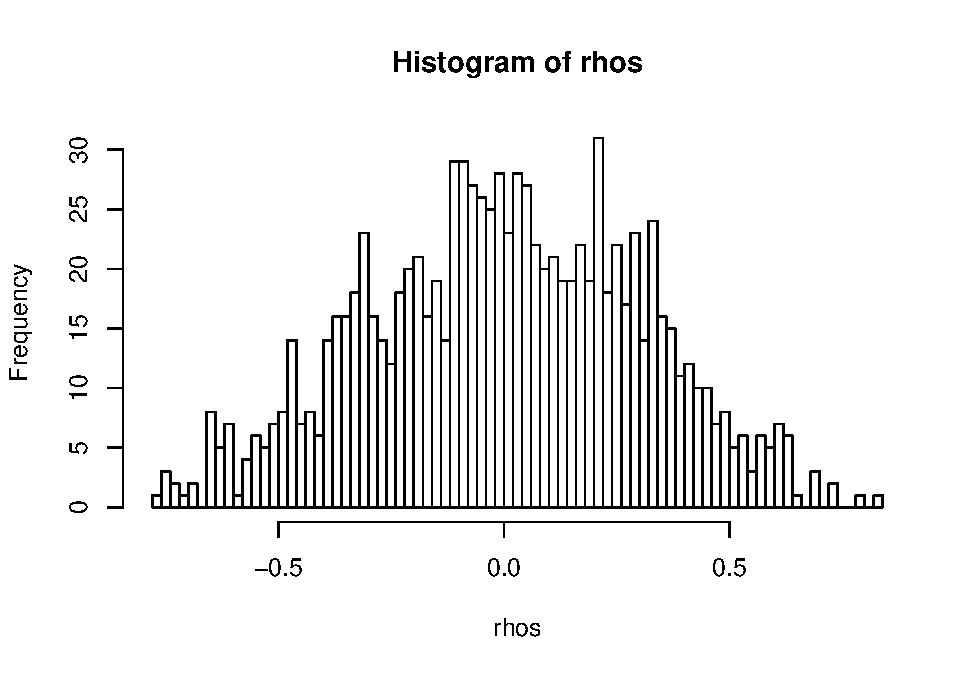
\includegraphics{428HW5-yutingd3_files/figure-latex/unnamed-chunk-18-1.pdf}

\begin{Shaded}
\begin{Highlighting}[]
\NormalTok{(}\DataTypeTok{theta.hat =}\NormalTok{ spearman.cor.test}\OperatorTok{$}\NormalTok{estimate)}
\end{Highlighting}
\end{Shaded}

\begin{verbatim}
## rho 
##   1
\end{verbatim}

\begin{Shaded}
\begin{Highlighting}[]
\NormalTok{spearman.cor.test}\OperatorTok{$}\NormalTok{p.value}
\end{Highlighting}
\end{Shaded}

\begin{verbatim}
## [1] 0
\end{verbatim}

\begin{Shaded}
\begin{Highlighting}[]
\NormalTok{(}\DataTypeTok{p.hat =} \KeywordTok{mean}\NormalTok{(}\KeywordTok{abs}\NormalTok{(rhos) }\OperatorTok{>}\StringTok{ }\KeywordTok{abs}\NormalTok{(theta.hat)))}
\end{Highlighting}
\end{Shaded}

\begin{verbatim}
## [1] 0
\end{verbatim}

\begin{Shaded}
\begin{Highlighting}[]
\NormalTok{(}\DataTypeTok{alpha =} \FloatTok{0.05}\NormalTok{)}
\end{Highlighting}
\end{Shaded}

\begin{verbatim}
## [1] 0.05
\end{verbatim}

\begin{Shaded}
\begin{Highlighting}[]
\CommentTok{# p.hat < alpha, thus H0 rejected.}
\end{Highlighting}
\end{Shaded}

\end{document}
